% Method overview (TikZ). \input by main.tex inside a figure environment.
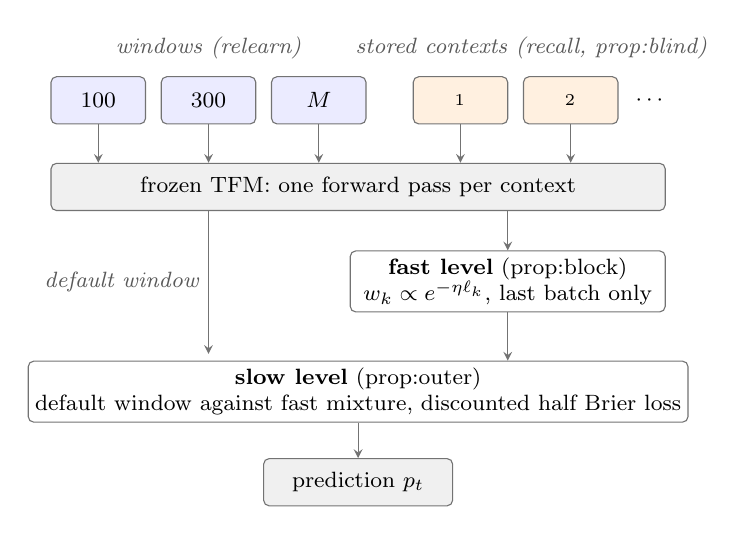
\begin{tikzpicture}[font=\footnotesize, >=stealth,
    box/.style={draw=black!55, rounded corners=2pt, minimum height=6mm, inner sep=2.5pt, align=center, fill=#1},
    box/.default=white,
    lab/.style={font=\footnotesize\itshape, text=black!65}]
  % experts
  \node[box=blue!8, minimum width=12mm] (w1) at (0,0)      {100};
  \node[box=blue!8, minimum width=12mm] (w2) at (1.4,0)    {300};
  \node[box=blue!8, minimum width=12mm] (w3) at (2.8,0)    {$M$};
  \node[box=orange!12, minimum width=12mm] (s1) at (4.6,0) {$\cC_1$};
  \node[box=orange!12, minimum width=12mm] (s2) at (6.0,0) {$\cC_2$};
  \node at (7.0,0) {$\cdots$};
  \node[lab, anchor=south] at (1.4,0.4) {windows (relearn)};
  \node[lab, anchor=south] at (5.5,0.4) {stored contexts (recall, \cref{prop:blind})};
  % frozen TFM
  \node[box=black!6, minimum width=78mm] (tfm) at (3.3,-1.1) {frozen TFM: one forward pass per context};
  \foreach \n in {w1,w2,w3,s1,s2} \draw[->, black!55] (\n.south) -- (\n.south |- tfm.north);
  % fast level (to the right of the default arrow)
  \node[box=white, minimum width=40mm] (fast) at (5.2,-2.3)
       {\textbf{fast level} (\cref{prop:block})\\ $w_k\propto e^{-\eta\ell_k}$, last batch only};
  \draw[->, black!55] (tfm.south -| fast.north) -- (fast.north);
  % slow level
  \node[box=white, minimum width=78mm] (slow) at (3.3,-3.7)
       {\textbf{slow level} (\cref{prop:outer})\\ default window against fast mixture, discounted half Brier loss};
  \draw[->, black!55] (fast.south) -- (fast.south |- slow.north);
  \draw[->, black!55] (1.4,-1.4) -- node[left, lab] {default window} (1.4,-3.22);
  \node[box=black!6, minimum width=24mm] (out) at (3.3,-4.85) {prediction $p_t$};
  \draw[->, black!55] (slow.south) -- (out.north);
\end{tikzpicture}
